\section{System Requirements}

Requirement planning and Hazard Analysis has always been a vital process in the development of mission-critical systems. In the automotive, marine, aerospace and military technology industries several Funstional Safety standards exist to guide the development and verification procedures, and ensure that the final product meets a certain quality and level of reliability. Losing or sinking the prototype due to faulty design or construction would have a devastating effect on my thesis, therefore I treated the system as mission-critical, trying to ensure very high reliability. Myí goal isn't the full compliance to all possible safety regulations, but there are some well designed procedures in these standards that can enhance the quality and reveal certain problems that can be dealth width before they become hazards.

\subsection{General guidelines}

Defining the general requirements of the system, especially without a hard functional requirement system, or we could say "out of thin air" is not straightforward. A good entrance to the world of Unmanned surface Vehicles is a document\cite{usvmasterplan} published by the DoN about general recommendations to companies developing Unmanned Surface Vehicles. According to the document, the requirements for developing autonomous boats for the US-Navy can be summarized in the following points:

\begin{enumerate}
	\item Align to the 4 classes of vehicles, with common core systems and interfaces to the greatest degree possible. Comply with the PEO-LMW-chartered and industry-led unmanned systems standards being developed. Standardize the vehicle interface to the host as well as within the vehicle, with standards for each class and common vehicle functions leveraged among different classes.
	\item Wean from the bandwidth. Greater autonomy must be developed to reduce data requirements sent “to” the USV, and more advanced automated target recognition must be developed to reduce the data requirements “from” the USV.
	\item Invest in a balanced USV technology program, that includes autonomy, collision avoidance, coupled payloads / weapons, launch / recovery and advanced hull / mechanical / electrical systems
	\item Ensure manual, semi-autonomous and autonomous operation modes, but concentrate on manual operation first
	\item In case of weaponized systems, investigate and apply the rules of maritime law and laws of war
	\item Continously deploy modules to receive operator feedback. Develop with consistent navy guidance. Continue the outreach to Navy operational, doctrine, and training commands to expand and refine employment concepts for USVs
\end{enumerate}

\paragraph{(1.)} is only slightly relevant. Alignment to the navy classes in not important, but a standardization of the interfaces is advantageous.
Therefore the control system should be designed for a general mobile robotic system, not ship-specific. The map and environment should be extendable to the third dimension, and must be able to track changes over time. The tasks of the low level control must be as specific and as basic as possible. All calculations and control should be implemented in the high level controller. Certain modules of the high level controller must be parametrized, dependent on the low level and hardware characteristics.

The point of these guidelines is to create a system of components with high reusability. Ideally a general Cross-platform High Level Controller controls different kind of vessels, through a standard interface. When changing to a different vehicle, only the Low Level Controller must be replaced, which stores the characteristics of the vessel and implements the actuator control.

\paragraph{(2.)} is a major guideline in the development of all unmanned systems. Compliance to the highest level should be sought.

\paragraph{(3.)} is very important in production systems, but the current area of application is academic. Ensuring a balanced technology would result in unsutainable amount of work, therefore already available consumer products and rapid prototyping technologies are used to great extent, wherever possible.

\paragraph{(4.)} Straightforward, complex features should be introduced gradually. More information about the operation modes in its respective subsection.

\paragraph{(5.)} Weaponization is not in the scope of the thesis.

\paragraph{(6.)} The academic environment ensures a certain level of feedback. In addition, contact with military and civilian naval personell is planned.

\subsection*{Operation models}

A typical oceanography application starts on the shore. A science team analyzes the currently available data, then marks the area of measurements on the map. The  map data is transformed to a measurement path by the scientists or by the automatic waypoint planner of the ship. The autonomous surface vehicle is then outfitted with the right sensors for the task, and a manned ship transports it close to its destination. The crew can set the research vessel to manual, automatic or fully autonomous mode.

\paragraph{Manual control}
In this mode it's possible for the operator to control the movement of the ship in world or body coordinates, like an industrial robot, or the actuators themselves. The primary intent of this mode is for testing and recovery.

\begin{figure}[H]
	\centering
	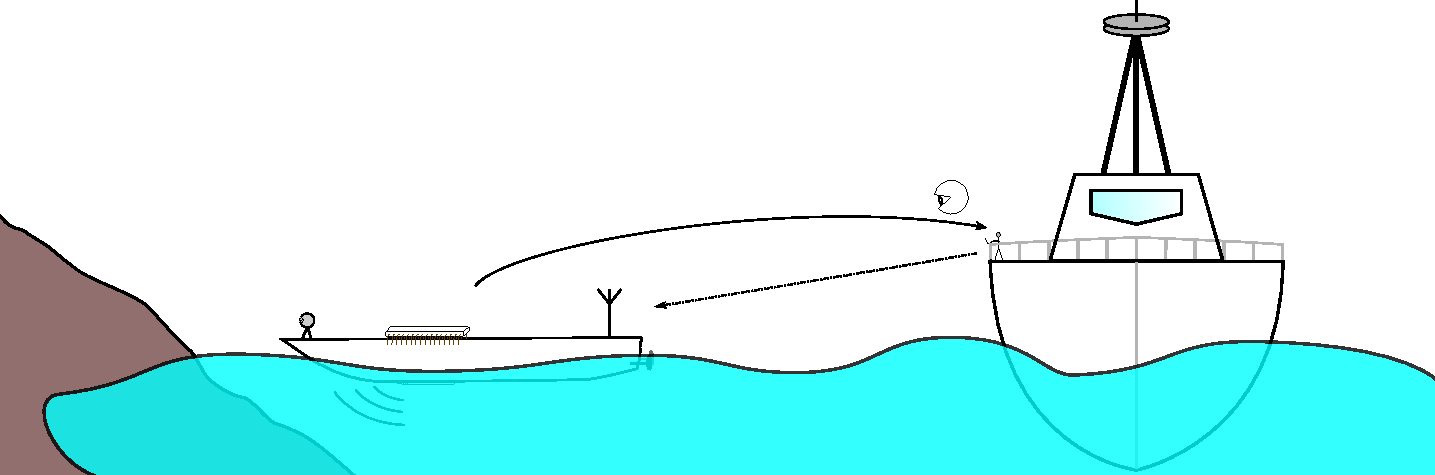
\includegraphics[width=0.8\textwidth]{img/manualcontrol}
	\caption{Manual remote control}
	\label{fig:manualcontrol}
\end{figure}

\paragraph{Semi-autonomous (automatic) control}
In automatic mode the "brains", remain on the manned vessel, and the research craft remains in wireless connection with the Mothership. When the measurements are complete, the oceanographer returns to the mothership. In automatic mode it is always possible to switch to manual control and back, or update the measurement path, etc.

\begin{figure}[H]
	\centering
	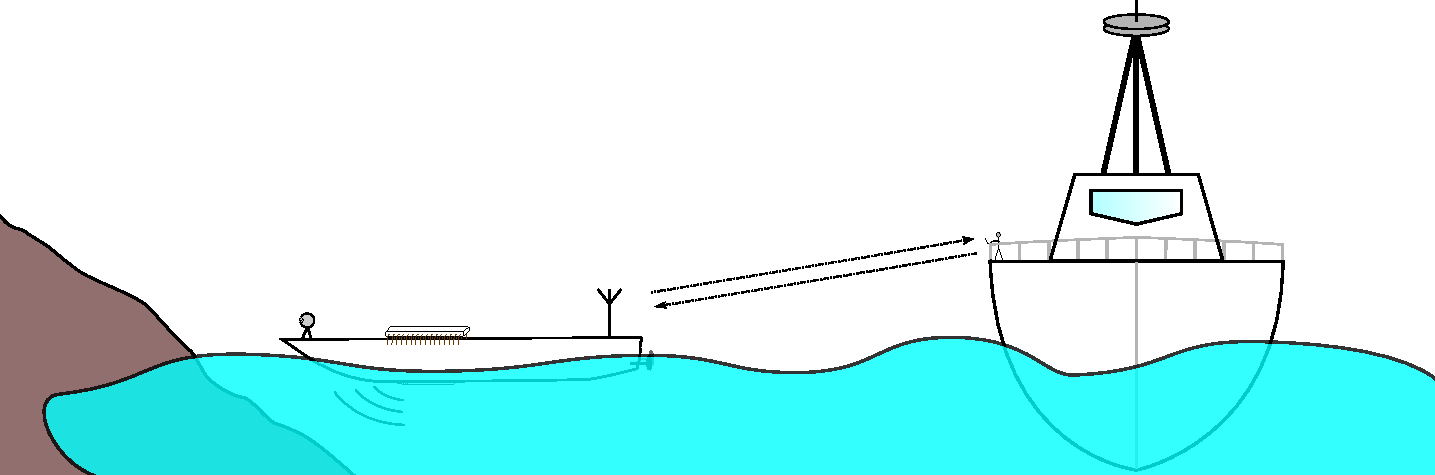
\includegraphics[width=0.8\textwidth]{img/automatic}
	\caption{Automatic supervised control}
	\label{fig:automatic}
\end{figure}

\paragraph{Autonomus control}
In Autonomus mode the ship carries everything that is needed to complete the task. Connection to the mothership can be cut, and the vessel carries the orders out autonomusly. Intervention in this mode is only possible until the oceanographer is in range of the mothership, or a special long range radio or satellite link can be installed to provide a low-bandwidth, but constant connection.

\begin{figure}[H]
	\centering
	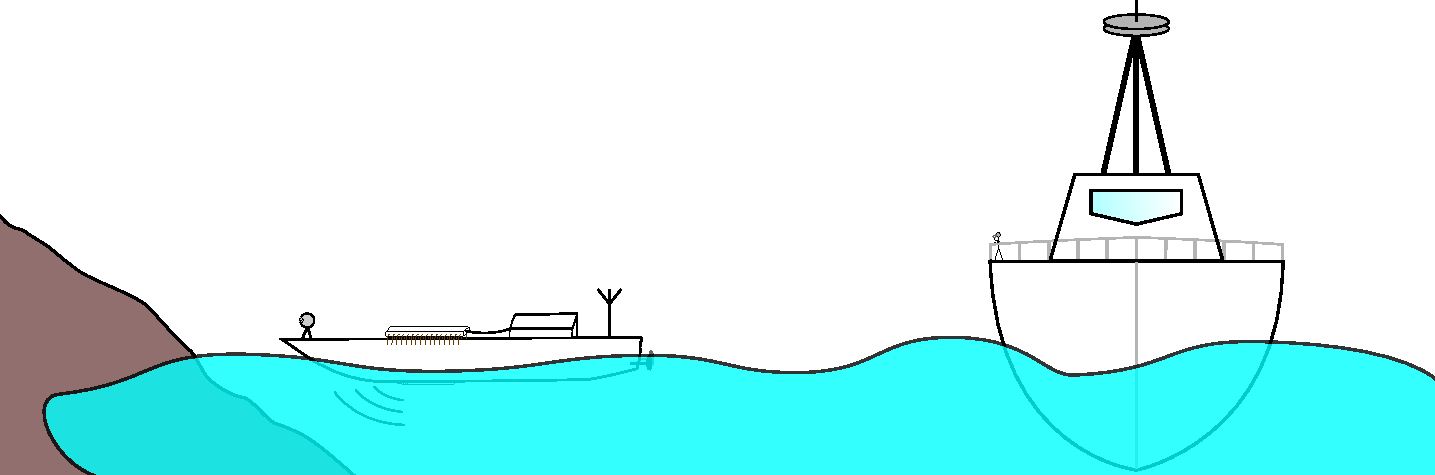
\includegraphics[width=0.8\textwidth]{img/autonomus}
	\caption{Autonomus control}
	\label{fig:autonomus}
\end{figure}

\paragraph{Squadron mode}
In case there are multiple research vessels, they can form a squadron. In this setup only one of the ships needs to be in range of the crewed mothership to control all of them, as each ship can function as a range-extender unit. Alternatively, one autonomous craft outfitted width long-range communication can control other crafts in automatic mode, taking over the role of the mothership, overseeing and planning the actions of the swarm.

\begin{figure}[H]
	\centering
	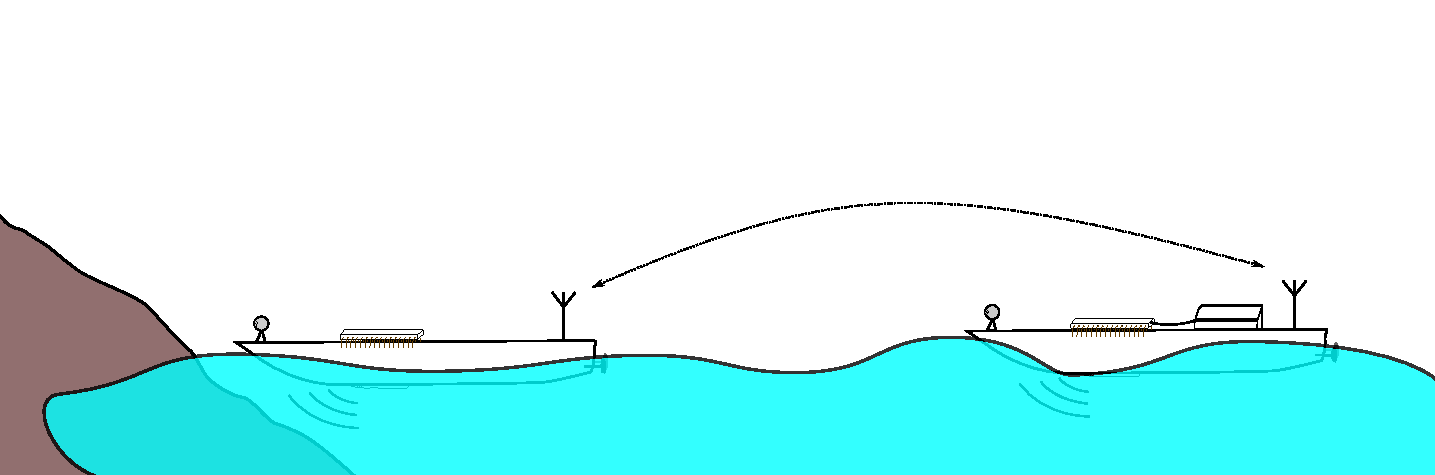
\includegraphics[width=0.8\textwidth]{img/multiple}
	\caption{Squadron mode}
	\label{fig:multiple}
\end{figure}

\begin{tcolorbox}[colback=cyan!5,colframe=cyan!40!black,title=Code: Main.py \\ https://www.dropbox.com/s/h1067ywmdajkegk/Main.py]
\begin{minipage}{0,6\textwidth}
The mission planning steps are implemented in Main.py, which is the main part of the program, responsible for initializing the system, setting the target area, mode of routing, navigation, etc. Later Main.py will provide a Graphical User Interface as well.
\end{minipage}
\begin{minipage}{0,35\textwidth}
\raggedleft

\includegraphics[width=0.8\textwidth]{img/main}
\end{minipage}

\end{tcolorbox}

\subsection{Navigational requirements of mobile robots}

Due to the fact that mobile robots are operating in a constantly changing environment, they must meet certain requirements. The most basic operational requirements can be summarized\cite{navreq}, and thus provide a basis for the navigation amd pathplanning algorithm:

\begin{itemize}
\item Convergence
\begin{itemize}
	\item The robot must reach the target in finite time, or
	\item If the robot is unable to reach the target, it must recognize this in finite time
\end{itemize}
\item Learning
\begin{itemize}
	\item The robot must learn its environment during the navigation
	\item Creation of maps, obstacles and Feasible Free Space
\end{itemize}
\item Monotonity
\begin{itemize}
	\item The shortest route to the target must not increase during movement and learning
\end{itemize}
\item Algorithm
\begin{itemize}
	\item The navigation algorithm must not limit the complexity of the environment
	\item The environmental dependency of the algorithm must be minimal
\end{itemize}

\end{itemize}

The verification of the navigation module is implemented in Python, as a general mobile robot pathplanning problem. A more complex approach is the 

\begin{figure}[H]
	\centering
	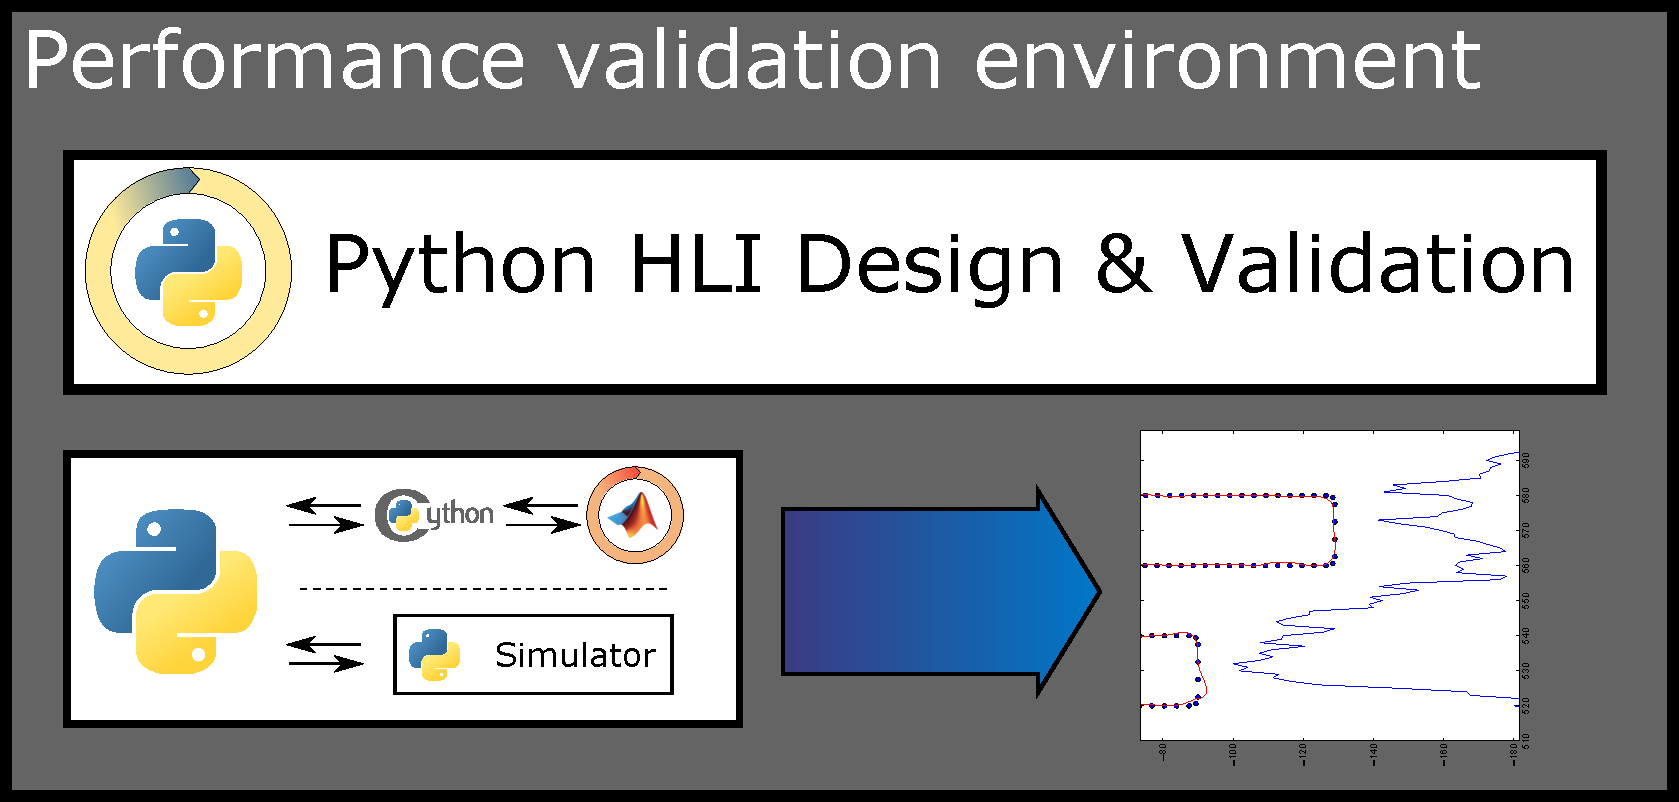
\includegraphics[width=0.8\textwidth]{img2/HLIVali}
	\caption{}
	\label{}
\end{figure}

\subsection{Software requirements of the system}

TODO, based on criticality of systems

\subsection{Requirements of survey ships}

In order to execute a rational oceanography task, a number of valid objectives must be set. These objectives are usually one or more of the following\cite{oceanography}:

\begin{itemize}
\item A set of geographical measurement locations, with or without time and measurement type conditions
\item A certain area of interest
\item Maximal action duration requirement
\item Other
\end{itemize}

The task planning is usually carried out by the scientist group, but some auto-planning modes need to be supported. A typical task is the creation of a measurement-grid, with preset definition, in a certain geographical area. The High Level Controller (HLC) uses a Mission planning time algorithm, to support the auto-generation of the waypoints. This module is the "Waypoint planner", which outputs a list of coordinates that contains the measurement points. The Waypoint planner must be operable during the execution of the mission, so a system reset will not cause termination.

\subsection{Requirements of the control system}

Every ship must meet certain maneuvering requirements\cite[p. 53]{hydromechanics}. They must possess course stability, as they must be able to maintain a direction or course. The drift angle, which is the angle between the heading and the actual course of the ship must also not show large fluctuations. The ship must be able to change course relatively fast, without significant overshoot, and the path width must be limited. The ship must also be able relatively well to accelerae and come to a full stop, and must remain well maneuverable during this time. Also, the ship must be able to maneuver with low speeds as well.

Translating these requirements to the language of a control engineer results in the following points:

\begin{itemize}

\item The controller can effectively estimate the current state of the ship
\item The controller ensures the asymptotic stability of the closed-loop system for all controllable states and all possible inputs

\end{itemize}

The control system will be developed in MATLAB-Simulink using the guidelines of the Model Based Design approach.
\begin{figure}[H]
	\centering
	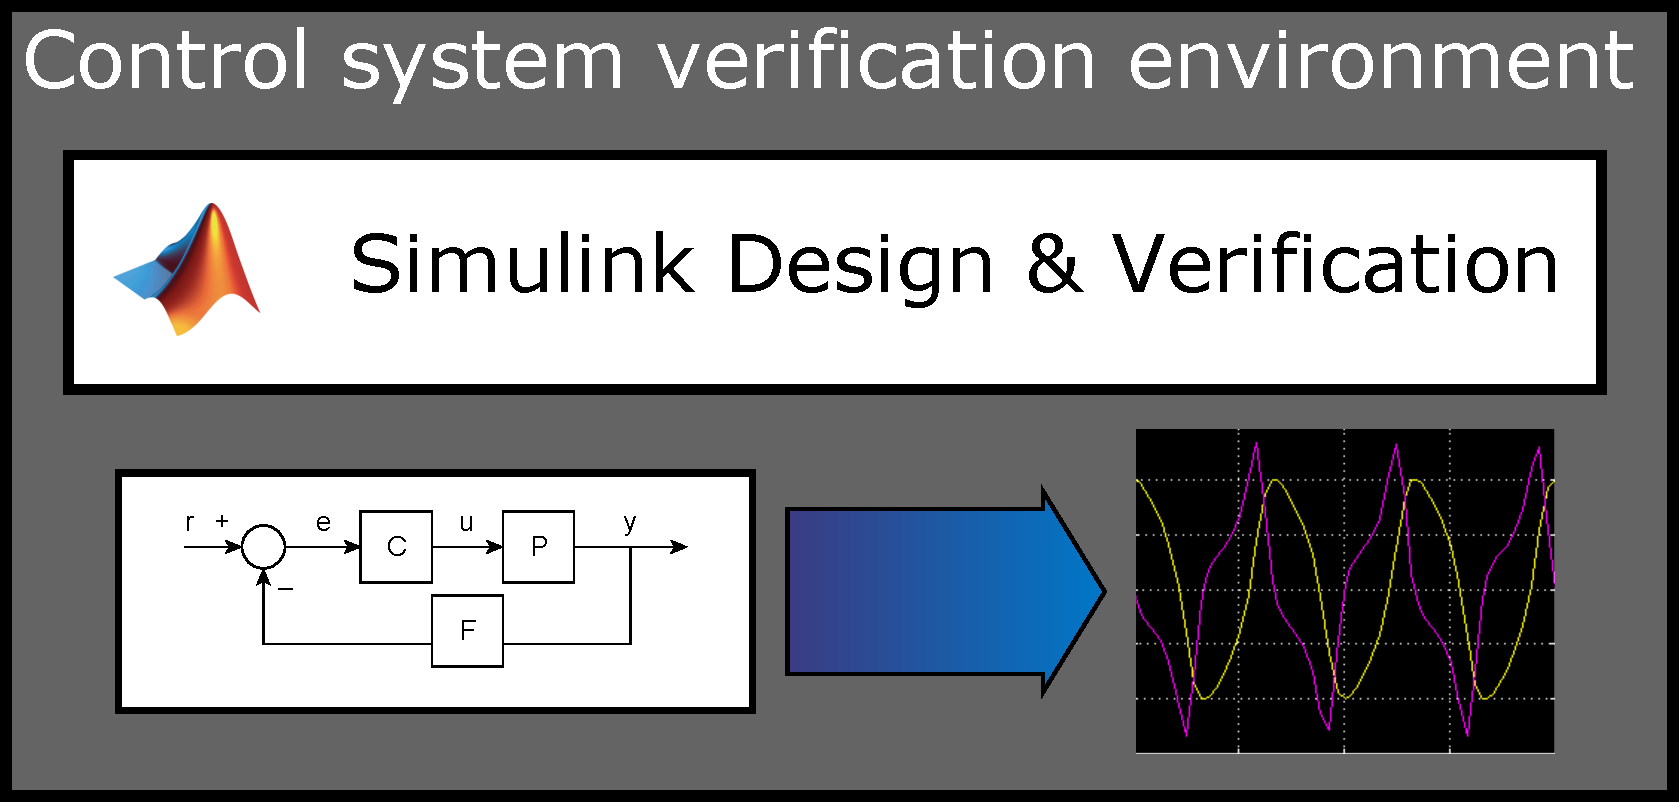
\includegraphics[width=0.8\textwidth]{img2/SimVer}
	\caption{Control system design and verification}
	\label{simver}
\end{figure}

Requirements of the communication:

TODO

\begin{itemize}

\item The module can transmit and receive serial Bluetooth data
\item The module can automatically re-establish connection with the slave Bluetooth devices (GPS and client)

\end{itemize}

\subsection{Requirements of the client software module}

TODO

\begin{itemize}

\item The client can transmit and receive serial Bluetooth data
\item The client can provide valid real-time information about the system
\item The client can automatically re-establish connection with the master Bluetooth device (HLI)

\end{itemize}

\begin{figure}[H]
	\centering
	
\includegraphics[width=0.6\textwidth]{img2/VeriBadges}
	\caption{}
	\label{}
\end{figure}